\chapter{闲谈\LaTeX 环境差异}\label{ch:environment}

%——————————————————————————————————%

\section{行间公式环境}
\Verb"\usepackage{amsmath}"

行间公式常用的有两种,一是 \textcolor{red!50!black}{\Verb"align"} 环境,另外一种是 \textcolor{red!50!black}{\Verb"equation"}环境。当两种环境都不带标号的时候,显示效果是一样的:
\begin{itemize}
    \item \textcolor{red!50!black}{\Verb"align*"}:
    \begin{align*}
        \hat{H} \Psi = \mathrm{i} \hbar \frac{\partial}{\partial t} \Psi.
    \end{align*}
    \item \textcolor{red!50!black}{\Verb"equation*"}:
    \begin{equation*}
        \hat{H} \Psi = \mathrm{i} \hbar \frac{\partial}{\partial t} \Psi.
    \end{equation*}
\end{itemize}
区别在于 \textcolor{red!50!black}{\Verb"align"}可以分行,而单用\textcolor{red!50!black}{\Verb"equation"}则不能分行:
\begin{itemize}
    \item \textcolor{red!50!black}{\Verb"align*"}:
    \begin{align*}
        \hat{H} \Psi & = \mathrm{i} \hbar \frac{\partial}{\partial t} \Psi \\
        \hat{H} \Psi & = E \Psi.
    \end{align*}
\end{itemize}
但如果想要进行公式编号,单用\textcolor{red!50!black}{\Verb"align"}环境会使得每一行都添加编号,显得很搞笑:
\begin{itemize}
    \item \textcolor{red!50!black}{\Verb"align"}:
    \begin{align}
        \hat{H} \Psi & = \mathrm{i} \hbar \frac{\partial}{\partial t} \Psi \\
        \hat{H} \Psi & = E \Psi \\
        \left( \hat{T} + \hat{V} \right) \Psi & = E \Psi \\
        \left( - \frac{\hbar^2}{2 m} \nabla^2 + \hat{V} \right) \Psi & = E \Psi
    \end{align}
\end{itemize}
这个时候建议使用\textcolor{red!50!black}{\Verb"equation + aligned"}环境:
\begin{itemize}
    \item \textcolor{red!50!black}{\Verb"equation + aligned"}:
    \begin{equation}
    \begin{aligned}
        \hat{H} \Psi & = \mathrm{i} \hbar \frac{\partial}{\partial t} \Psi \\
        \hat{H} \Psi & = E \Psi \\
        \left( \hat{T} + \hat{V} \right) \Psi & = E \Psi \\
        \left( - \frac{\hbar^2}{2 m} \nabla^2 + \hat{V} \right) \Psi & = E \Psi    
        \end{aligned}
    \end{equation}
\end{itemize}
或者使用\textcolor{red!50!black}{\Verb"subequations + equation"}环境
\begin{subequations}
    \begin{equation}
    \begin{aligned}
        \hat{H} \Psi & = \mathrm{i} \hbar \frac{\partial}{\partial t} \Psi
    \end{aligned}
    \end{equation}
    \begin{equation}
    \begin{aligned}
        \hat{H} \Psi & = E \Psi \\
        \left( \hat{T} + \hat{V} \right) \Psi & = E \Psi \\
        \left( - \frac{\hbar^2}{2 m} \nabla^2 + \hat{V} \right) \Psi & = E \Psi    
        \end{aligned}
    \end{equation}
\end{subequations}
\textcolor{red!50!black}{\Verb"subequations + align"}
\begin{subequations}
    \begin{align}
        \hat{H} \Psi & = \mathrm{i} \hbar \frac{\partial}{\partial t} \Psi \\
        \hat{H} \Psi & = E \Psi \\
        \left( \hat{T} + \hat{V} \right) \Psi & = E \Psi \\
        \left( - \frac{\hbar^2}{2 m} \nabla^2 + \hat{V} \right) \Psi & = E \Psi    
    \end{align}
\end{subequations}

\begin{remark}
    注意使用公式环境的时候,里面\textcolor{red!50!black}{\Verb"begin"}和\textcolor{red!50!black}{\Verb"end"}之间一定要有内容,也不要有空行,不然会报错。
\end{remark}
\begin{remark}
    更多公式环境请查看\href{https://en.wikibooks.org/wiki/LaTeX/Mathematics}{Latex数学wiki}
\end{remark}
%——————————————————————————————————%

\section{表格环境}
\textcolor{red!50!black}{\Verb"tabular"}才是主体!但是只用\textcolor{red!50!black}{\Verb"tabular"}环境的话,整个表格是左对齐的:

\begin{tabular}{c|c|c|c|c|c}
\hline
     $x$ & $1$ & $2$ & $3$ & $4$ & $5$ \\ \hline
     $f(x) = x^2$ & $1$ & $4$ & $9$ & $16$ & $25$\\ \hline
\end{tabular}

此时需要配合\textcolor{red!50!black}{\Verb"center"}环境,且此时的表格标题需要使用\textcolor{red!50!black}{\Verb"\\captionof\{table\}\{标题\}"}~(\textcolor{red!50!black}{\Verb"\\usepackage\{caption\}"}):
\begin{center}
\captionof{table}{用表格法描述函数.}
\begin{tabular}{c|c|c|c|c|c}
\hline
     $x$ & $1$ & $2$ & $3$ & $4$ & $5$ \\ \hline
     $f(x) = x^2$ & $1$ & $4$ & $9$ & $16$ & $25$\\ \hline
\end{tabular}
\end{center}

或者配合可以自动排位的\textcolor{red!50!black}{\Verb"table"}环境,类似于word里面的{``}文字环绕模式{''},此时的表格标题用{\Verb"\caption{标题}"}即可:\newline
\begin{table}[h!]
\centering
\begin{tabular}{c|c|c|c|c|c}
\hline
     $x$ & $1$ & $2$ & $3$ & $4$ & $5$ \\ \hline
     $f(x) = x^2$ & $1$ & $4$ & $9$ & $16$ & $25$\\ \hline
\end{tabular}
\end{table}
有时候\textcolor{red!50!black}{\Verb"tabular"}环境中的字没有在一行内居中,此时控制符可以选择使用{\Verb"m{xcm}<\centering"} ,而过窄的行距可使用\newline  {\Verb"\renewcommand{\arraystretch}{倍数}"}来调整,例如:
\begin{table}[h!]
\renewcommand{\arraystretch}{1.4}
\centering
\caption{用表格法描述函数.}
\begin{tabular}{m{2cm}<\centering|m{2cm}<\centering|m{2cm}<\centering|m{2cm}<\centering|m{2cm}<\centering|m{2cm}<\centering}
\hline
     $x$ & $1$ & $2$ & $3$ & $4$ & $5$ \\ \hline
     $f(x) = x^2$ & $1$ & $4$ & $9$ & $16$ & $25$\\ \hline
\end{tabular}
\end{table}

上色:
\begin{center}
\begin{tabular}{|c|c|c|c|}
\hline
    {\cellcolor{blue!25} 缓冲溶剂} & {\cellcolor{blue!25}共轭酸碱对形式} &  {\cellcolor{blue!25} $pK_a$ } & {\cellcolor{blue!25} 缓冲范围 } \\ \hline
    \ch{HCOOH} --- \ch{NaOH} & \ch{HCOOH} --- \ch{HCOO^-} & 3.75 & 2.75 $\sim$ 4.75  \\ \hline
    \ch{CH_3COOH} --- \ch{CH_3COONa} & \ch{HAc} --- \ch{Ac^-} & 4.75 & 3.75 $\sim$ 5.75  \\ \hline
    \ch{NaH_2PO_4} --- \ch{Na_2HPO_3} & \ch{H_2PO_4^-} --- \ch{HPO_4^{2-}} & 7.21 & 6.21 $\sim$ 8.21  \\ \hline
    \ch{Na_2B_4O_7} --- \ch{HCl} & \ch{H_3BO_3} --- \ch{H_2BO_3^-} & 9.14 & 8.14 $\sim$ 10.14 \\ \hline
    \ch{NH_3. H_2O} --- \ch{NH_4Cl} & \ch{NH_4^+} --- \ch{NH_3} & 9.25 & 8.25 $\sim$ 10.25  \\ \hline
    \ch{NaHCO_3} --- \ch{Na_2CO_3} & \ch{HCO_3^-} --- \ch{CO_3^{2-}} & 10.25 & 9.25 $\sim$ 11.25  \\ \hline
    \ch{Na_2HPO_4} --- \ch{NaOH} & \ch{HPO_4^{2-}} --- \ch{PO_4^{3-}} & 12.66 & 11.66 $\sim$ 13.66  \\ \hline
\end{tabular}
\end{center}


合并列与合并行如 \Verb"\multicolumn" 和 \Verb"\multirow"(\Verb"\usepackage{multirow}"):
\begin{center}
\begin{tabular}{|c|c|c|c|c|}
\hline
    \multicolumn{2}{|c}{\cellcolor{blue!25} 起始浓度(mol$\cdot$dm$^{-3}$)} & \multicolumn{2}{|c|}{\cellcolor{blue!25}转化率(\%)} &  \cellcolor{blue!25} \\ \cline{1-4}
    \ch{C_2H_5OH} & \ch{CH_3COOH} & \ch{C_2H_5OH} & \ch{CH_3COOH} &\cellcolor{blue!25} \multirow{ -2}{*}{平衡常数 K}\\ \hline
    3.0 & 3.0 & 67 & 67 & 4.0 \\ \hline
    3.0 & 6.0 & 83 & 42 & 4.0 \\ \hline
    6.0 & 3.0 & 42 & 83 & 4.0 \\ \hline
\end{tabular}
\end{center}

\begin{remark}
    \textcolor{red!50!black}{\Verb"tabular"}是{``}文字环境{''},即里面的字体都是直体,上标下标需要用行间公式\textcolor{red!50!black}{\Verb"\$\$"}来启用
\end{remark}
\begin{remark}
    更高级的表格用法 请查看\href{https://en.wikibooks.org/wiki/LaTeX/Tables#Rows_spanning_multiple_columns}{Latex表格wiki}
\end{remark}
\begin{remark}
    更好优雅的画矩阵和表格的方法可参考\Verb"NiceMatrix"包:\href{https://ctan.math.washington.edu/tex-archive/macros/latex/contrib/nicematrix/nicematrix.pdf}{NiceMatrix}
\end{remark}
\begin{lastremark}
和\textcolor{red!50!black}{\Verb"table"}环境类似, \textcolor{red!50!black}{\Verb"array"}环境也有对齐的功能。但\textcolor{red!50!black}{\Verb"array"}只能在数学环境中如 \textcolor{red!50!black}{\Verb"align"} 和 \textcolor{red!50!black}{\Verb"equation"} 中使用。
\end{lastremark}



%——————————————————————————————————%

\section{图片环境}
\LaTeX 中图片主要有四类,分别为:
\begin{itemize}
    \item tikz 图: 作图方法:
    \begin{verbatim}
\begin{center}
    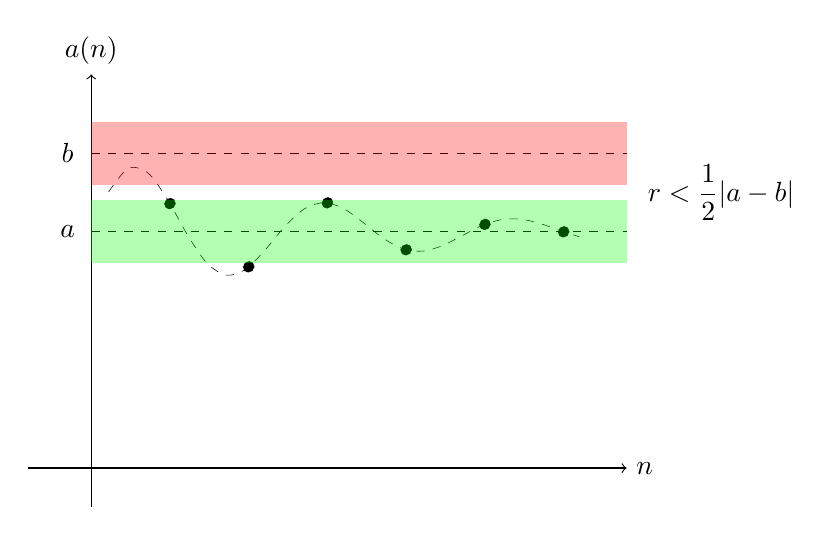
\begin{tikzpicture}
         %画数轴 / 画直线
        \draw[->] (-0.8,0) --(6.8,0) node[right] {$n$};
        \draw[->] (0,-0.5) --(0,5.0) node[above] {$a(n)$};
         
        \draw[dashed] (0, 4.0) -- (6.8,4.0) node at (-0.3, 4.0) {$b$};
        \draw[dashed] (0,3.0) -- (6.8, 3.0) node at (-0.3, 3.0){$a$};
        
        %画函数和点
        \draw[domain =0.22:6.2, variable=\x, dashed, very thin, smooth , black] 
        plot (\x ,{ exp(- \x / 3) * sin( 150 * \x) + 3 })  
        plot[only marks, mark=*, fill=black] coordinates
        {(1,3.3582657) (2,2.5553677) (3,3.3678794) (4,2.7717182) (5, 3.0944378) (6, 3)};
        
        %画简单封闭图形,只有封闭图形可以涂色;scope可以用来进行多种图形的组合,控制透明度等
        \begin{scope}[fill opacity=0.3]
            \fill[green] (0.0, 2.6) rectangle (6.8, 3.4) ;
            \fill[red] (0.0, 3.6) rectangle (6.8, 4.4) ;
        \end{scope}
        
        %添加标签
        \node at (8, 3.5) {$r <\dfrac{1}{2} |a - b|$}; 
        
    \end{tikzpicture}
\end{center}
    \end{verbatim}
\begin{center}
    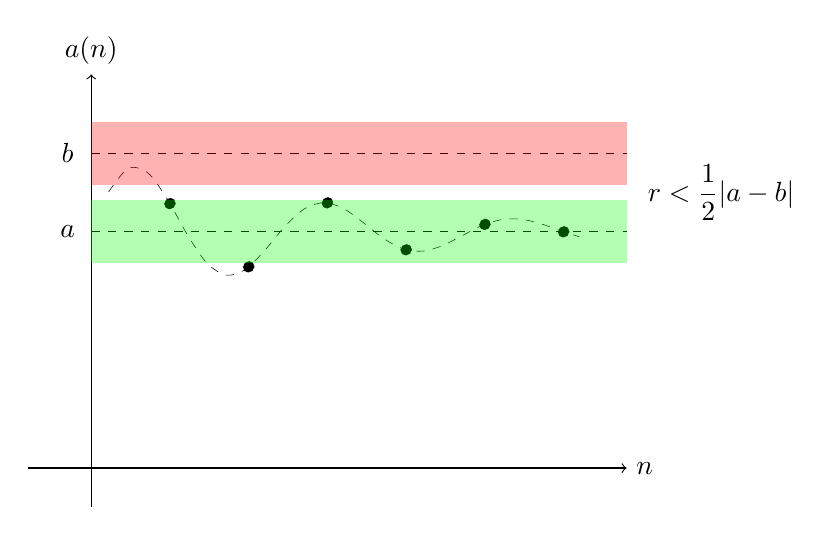
\begin{tikzpicture}
        \draw[->] (-0.8,0) --(6.8,0) node[right] {$n$};
        \draw[->] (0,-0.5) --(0,5.0) node[above] {$a(n)$};
        \draw[dashed] (0, 4.0) -- (6.8,4.0) node at (-0.3, 4.0) {$b$};
        \draw[dashed] (0,3.0) -- (6.8, 3.0) node at (-0.3, 3.0){$a$};
        \draw[domain =0.22:6.2, variable=\x, dashed, very thin, smooth , black] 
        plot (\x ,{ exp(- \x / 3) * sin( 150 * \x) + 3 })  
        plot[only marks, mark=*, fill=black] coordinates{(1,3.3582657) (2,2.5553677) (3,3.3678794) (4,2.7717182) (5, 3.0944378) (6, 3)};
        
        \begin{scope}[fill opacity=0.3]
            \fill[green] (0.0, 2.6) rectangle (6.8, 3.4) ;
            \fill[red] (0.0, 3.6) rectangle (6.8, 4.4) ;
        \end{scope}
        \node at (8, 3.5) {$r <\dfrac{1}{2} |a - b|$};        
    \end{tikzpicture}
    \captionof{figure}{例图1}
\end{center}
    \begin{lastremark}
    强烈推荐知乎里面tikz图的\href{https://zhuanlan.zhihu.com/p/127155579}{基础教程}.
    \end{lastremark}
    \item png 图: 导入方法:
    \begin{verbatim}
\begin{center}
    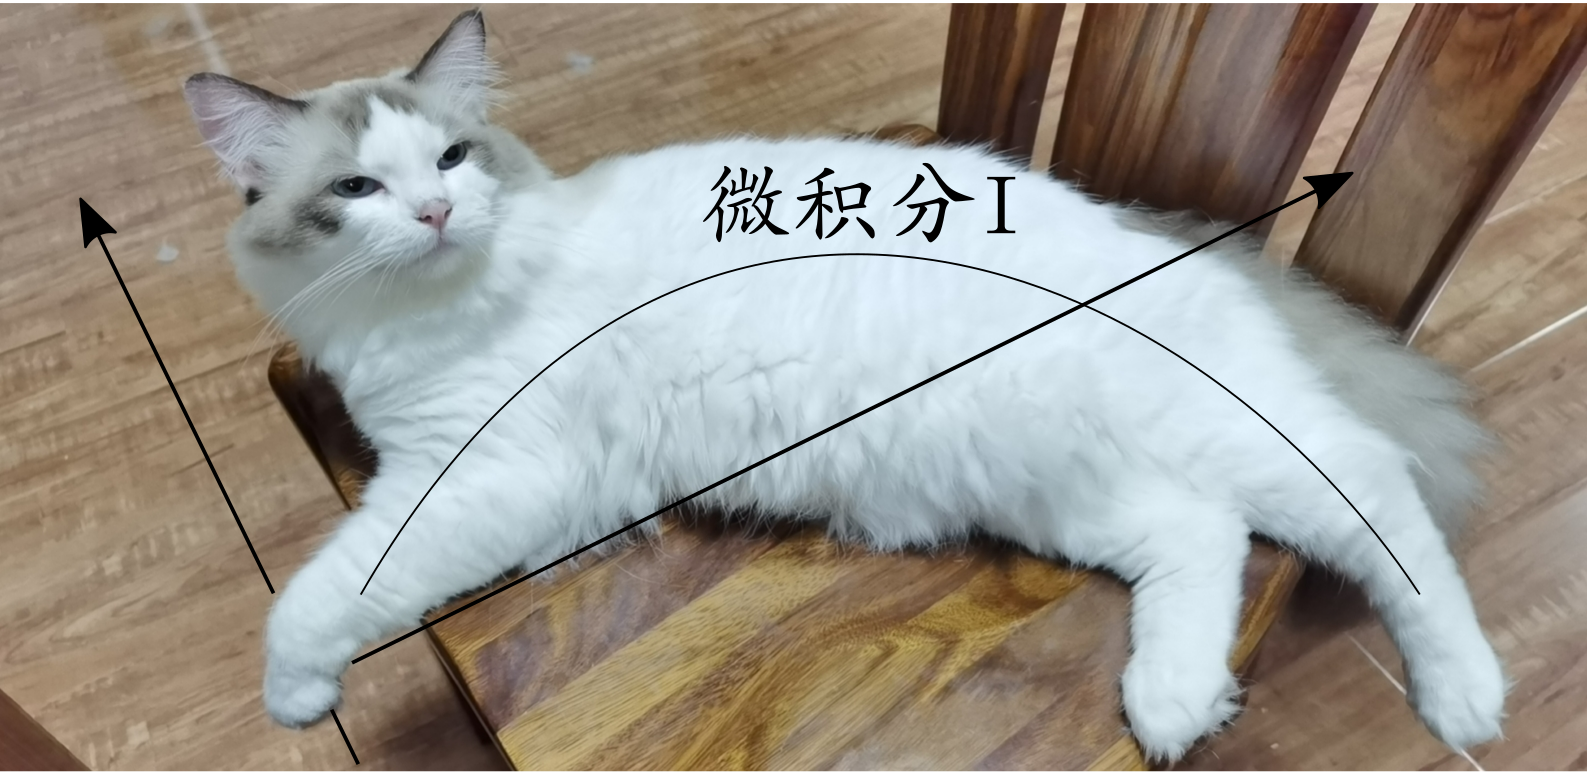
\includegraphics[scale=0.6]{figure/Ragdoll.png}
    \captionof{figure}{例图2}
\end{center}
    \end{verbatim}
    \begin{center}
    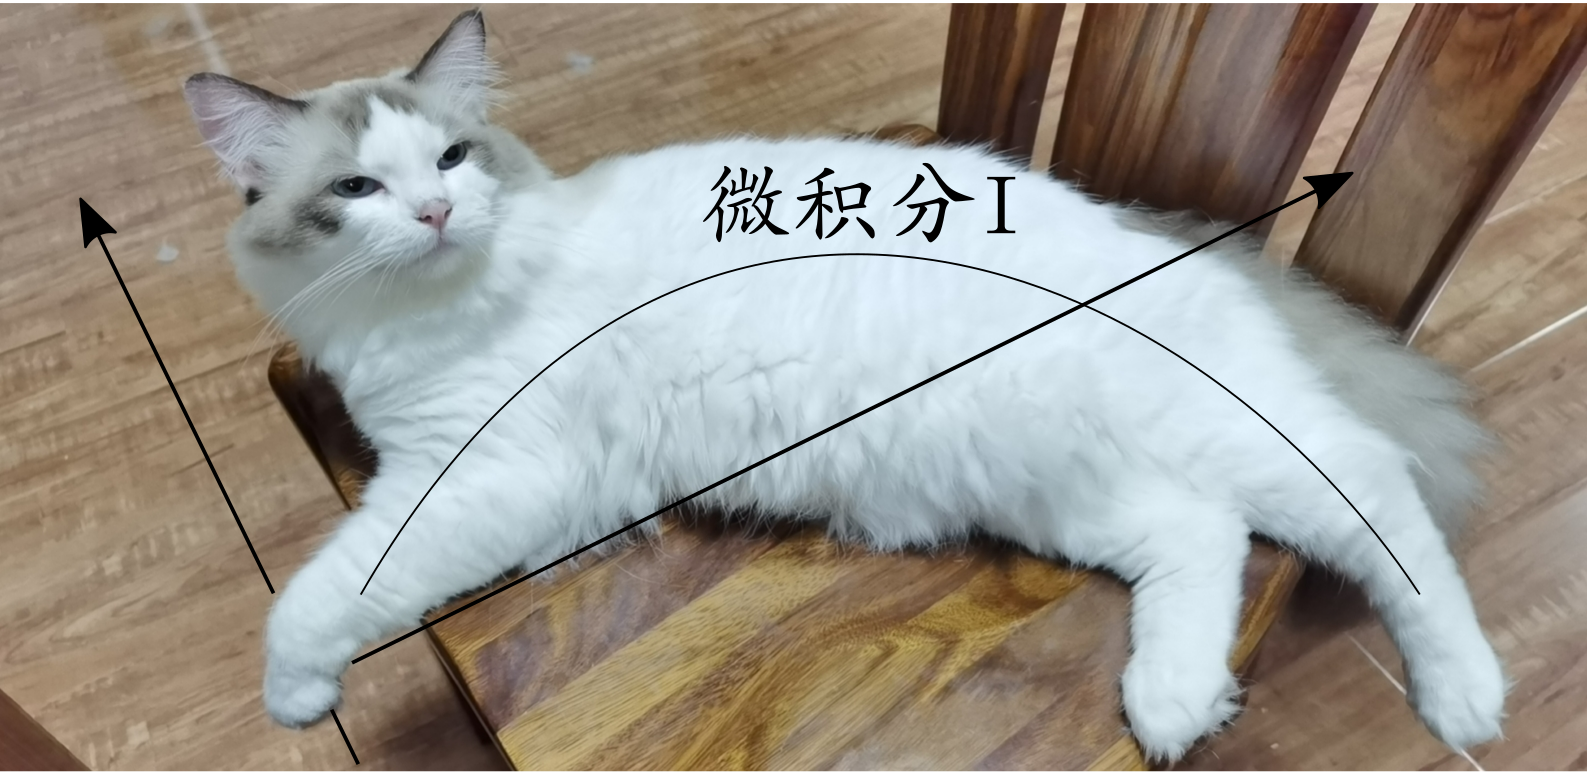
\includegraphics[scale=1]{figure/Ragdoll.png}
    \captionof{figure}{例图2}
    \end{center}
    \item svg 图:导入方法:
    \begin{verbatim}
\begin{center}
    \includesvg[scale=0.25]{figure/Ragdoll.svg}
    \captionof{figure}{例图3}
\end{center}        
    \end{verbatim}
    \begin{center}
    \includesvg[scale=0.25]{figure/Ragdoll.svg}
    \captionof{figure}{例图3}
    \end{center}   
    \item pdf 图 $+$ tex 文字: 导入方法:
    \begin{verbatim}
\begin{center}
    \def\svgwidth{0.7\columnwidth}
    \input{figure/Ragdoll.pdf_tex}
    \captionof{figure}{例图4.}
\end{center}
    \end{verbatim}
    \begin{center}
    \def\svgwidth{0.7\columnwidth}
    \input{figure/Ragdoll.pdf_tex}
    \captionof{figure}{例图4.}
    \label{fig:Ragdoll}
\end{center}
\end{itemize}
\begin{remark}
    强烈建议使用overleaf的用户在main.tex的同一个目录里面建立一个figure文件夹,然后把所有外部导入的图都放在里面。具体原因会在以后说明。
\end{remark}
\begin{remark}
    正如在表格环境中一样,上述例子中的\textcolor{red!50!black}{\Verb"center"}环境可以改为\textcolor{red!50!black}{\Verb"figure"}环境,而图片的标题则需要由\textcolor{red!50!black}{\Verb"captionof\{figure\}\{标题\}"}改为\textcolor{red!50!black}{\Verb"caption\{标题\}"}
\end{remark}






%——————————————————————————————————%

\section{分页环境}
\textcolor{red!50!black}{\Verb"minipage"} 环境是文字环境,在书本中的应用场景很少,主要应用于beamer和海报中.
\begin{proposition}
\begin{minipage}{0.5\textwidth}
莫比乌斯带是在平面$[0,1]\times[0,1]$中,规定了$(0,y) \sim (1,y)$后的商拓扑。
\end{minipage}
\begin{minipage}{0.5\textwidth}
    \begin{center}
    \includesvg[scale=0.6]{figure/mobius.svg}
    \end{center} 
\end{minipage}
\end{proposition}




%——————————————————————————————————%
